




\section{Scheduling for Multi-Class Queuing Networks: Benchmarks}
\label{section:results}


We now benchmark the performance of the policies obtained by $\pathwise$ policy gradient (Algorithm~\ref{alg:pathwise-pg}) with standard queuing policies and policies obtained using state-of-the-art model-free reinforcement learning algorithms.
We consider networks displayed in Figure~\ref{fig:networks}, which were briefly described in section~\ref{sec:gradient_efficiency} and appeared in previous works~\cite{dai2022queueing, bertsimas2014robust}. \citet{dai2022queueing} used Criss-cross and Re-entrant-1 networks to show that $\ppo$ can outperform standard queuing policies. \citet{bertsimas2014robust} consider the Re-entrant-2 network, but did not include any RL baselines. We consider networks with exponential inter-arrival times and workloads in order to compare with previous results. We also consider hyper-exponential distributions to model settings with higher coefficients of variation, as has been observed in real applications~\cite{green2007coping}. The hyper-exponential distribution $X\sim \mathsf{HyperExp}(\lambda_{1},\lambda_{2},p)$ is a mixture of exponential distributions:
\[
X \stackrel{d}{=} Y\cdot E_{1} + (1 - Y) \cdot E_{2},
\]
for $Y\sim\mathsf{Bernoulli}(p)$, $E_{1} \sim \mathsf{Exp}(\lambda_{1})$, $E_{2} \sim \mathsf{Exp}(\lambda_{2})$, and all are drawn independently of each other. We calibrate the parameters of the hyper-exponential distribution to have the same mean as the corresponding exponential distribution, but with a 1.5x higher variance.
\begin{figure}[t]
\centering
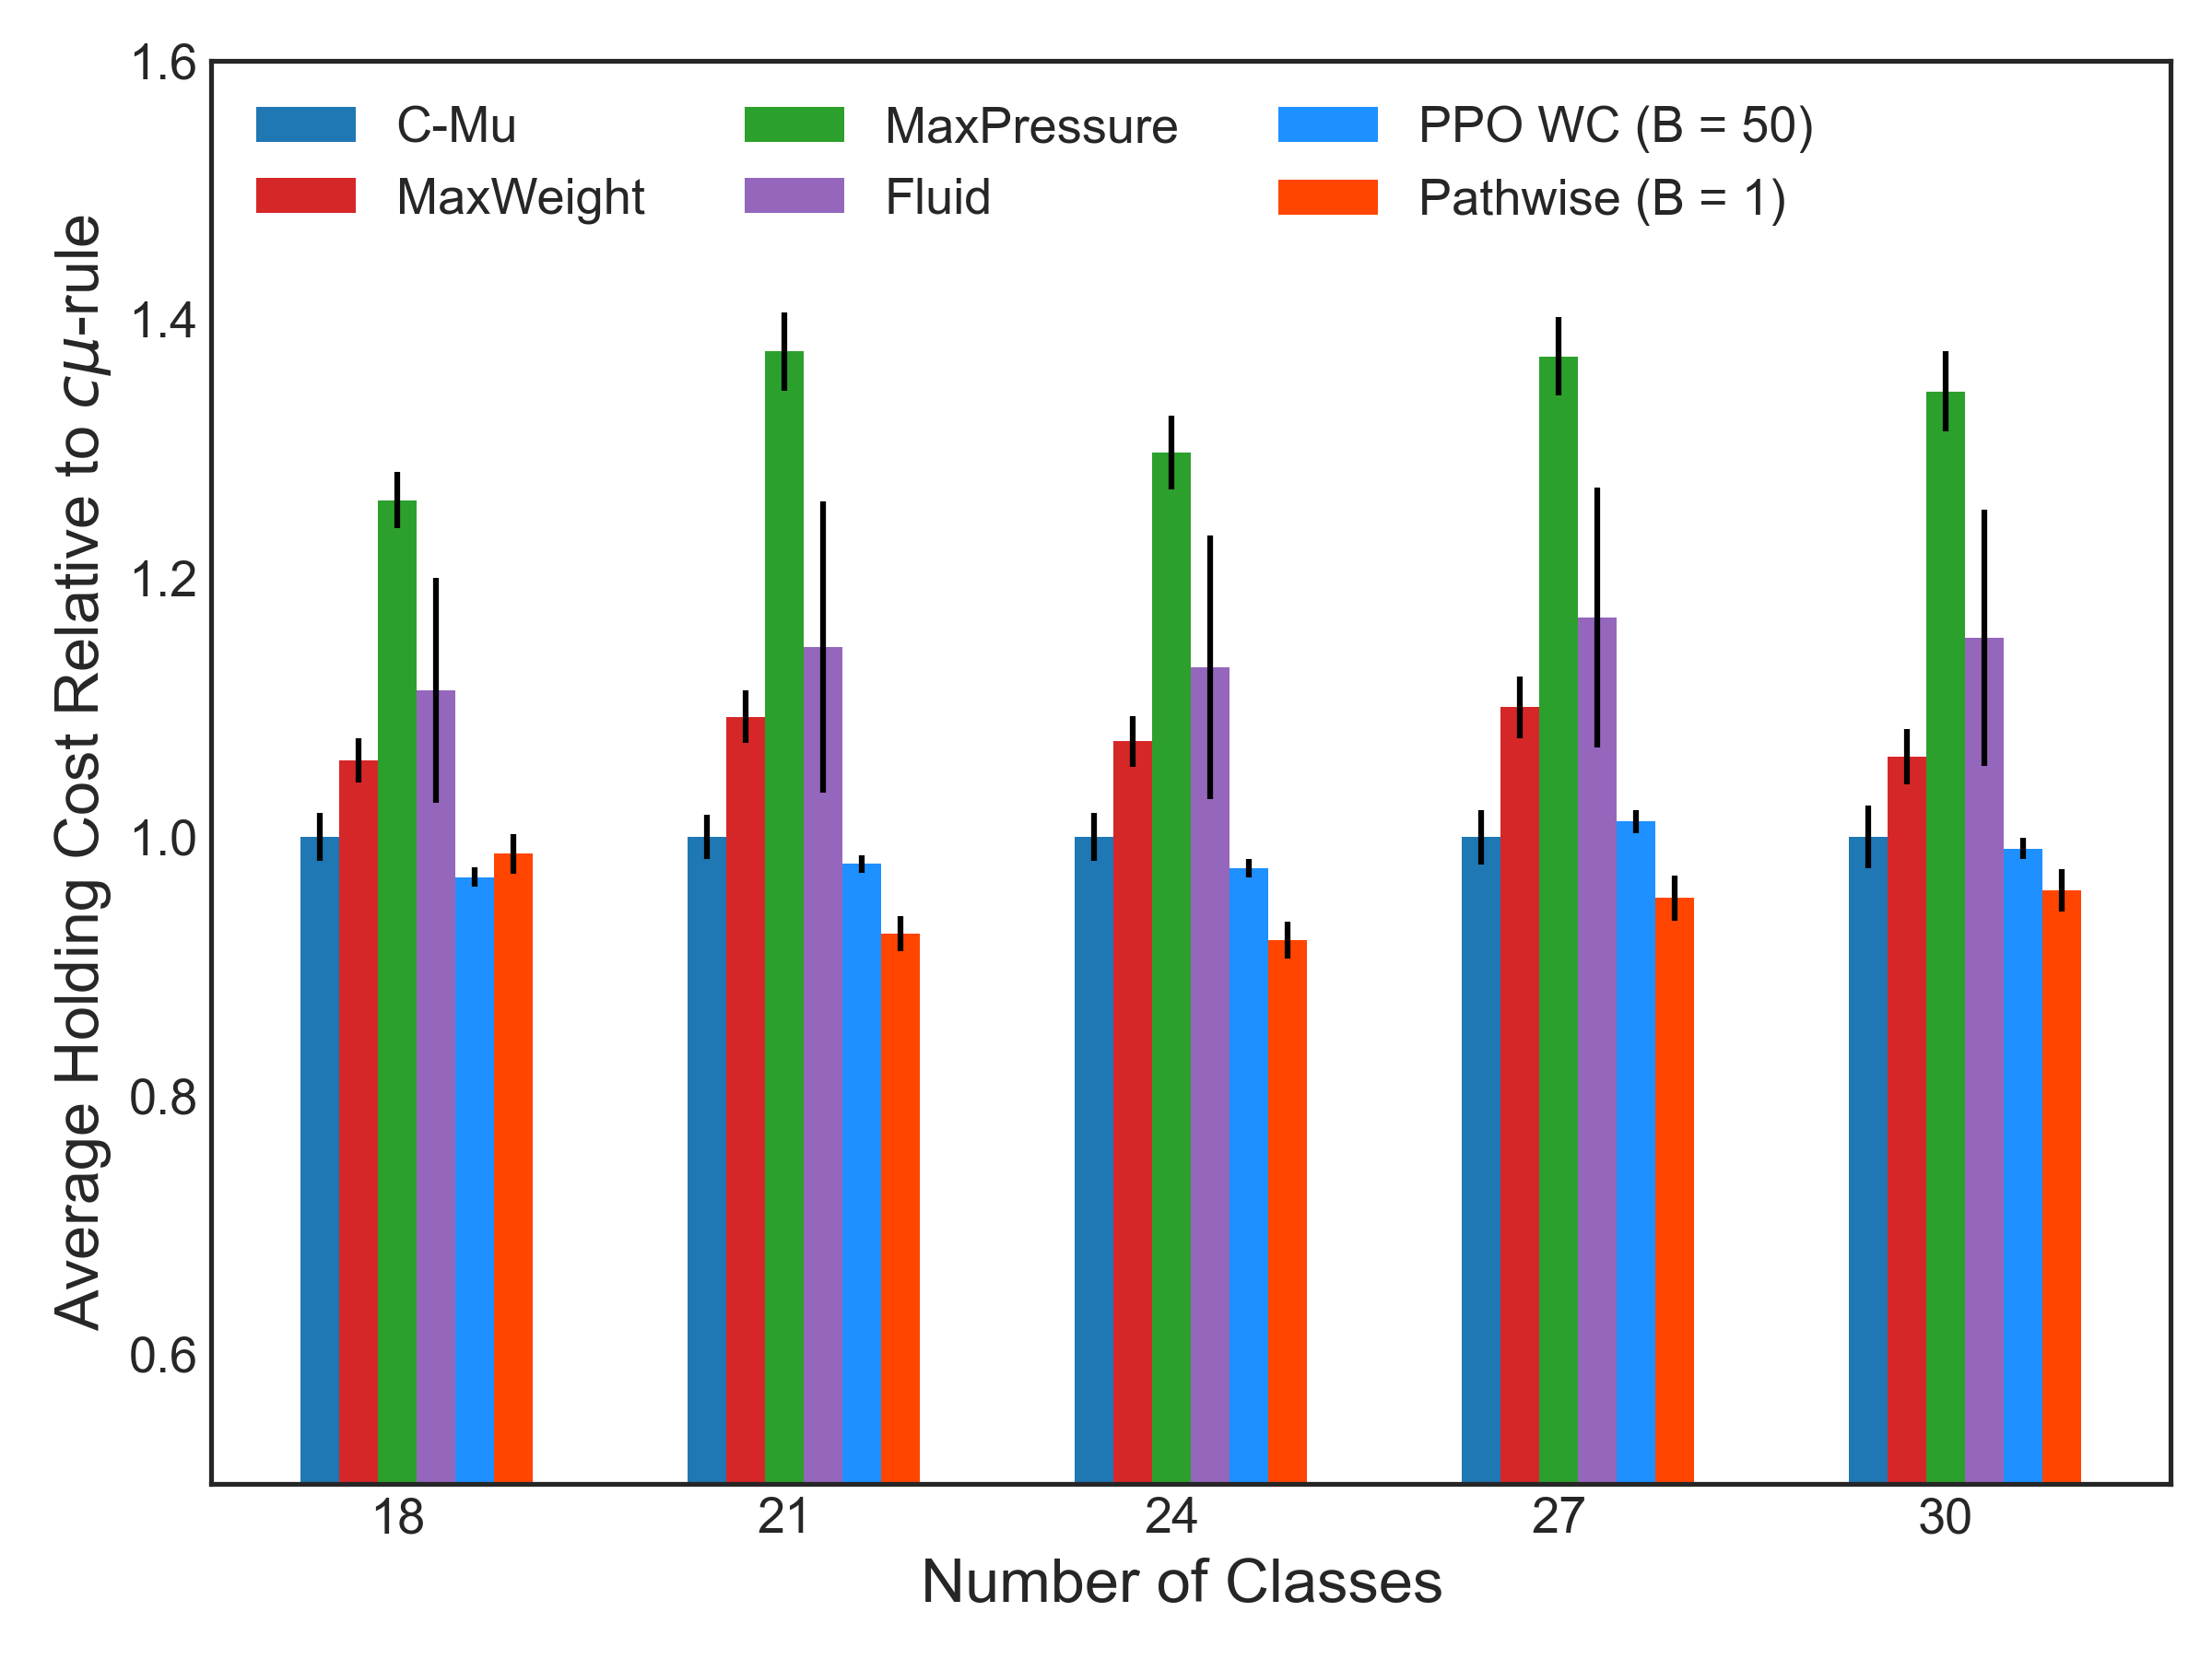
\includegraphics[height = 2.2in]{plot/results/reentrant_results.png}
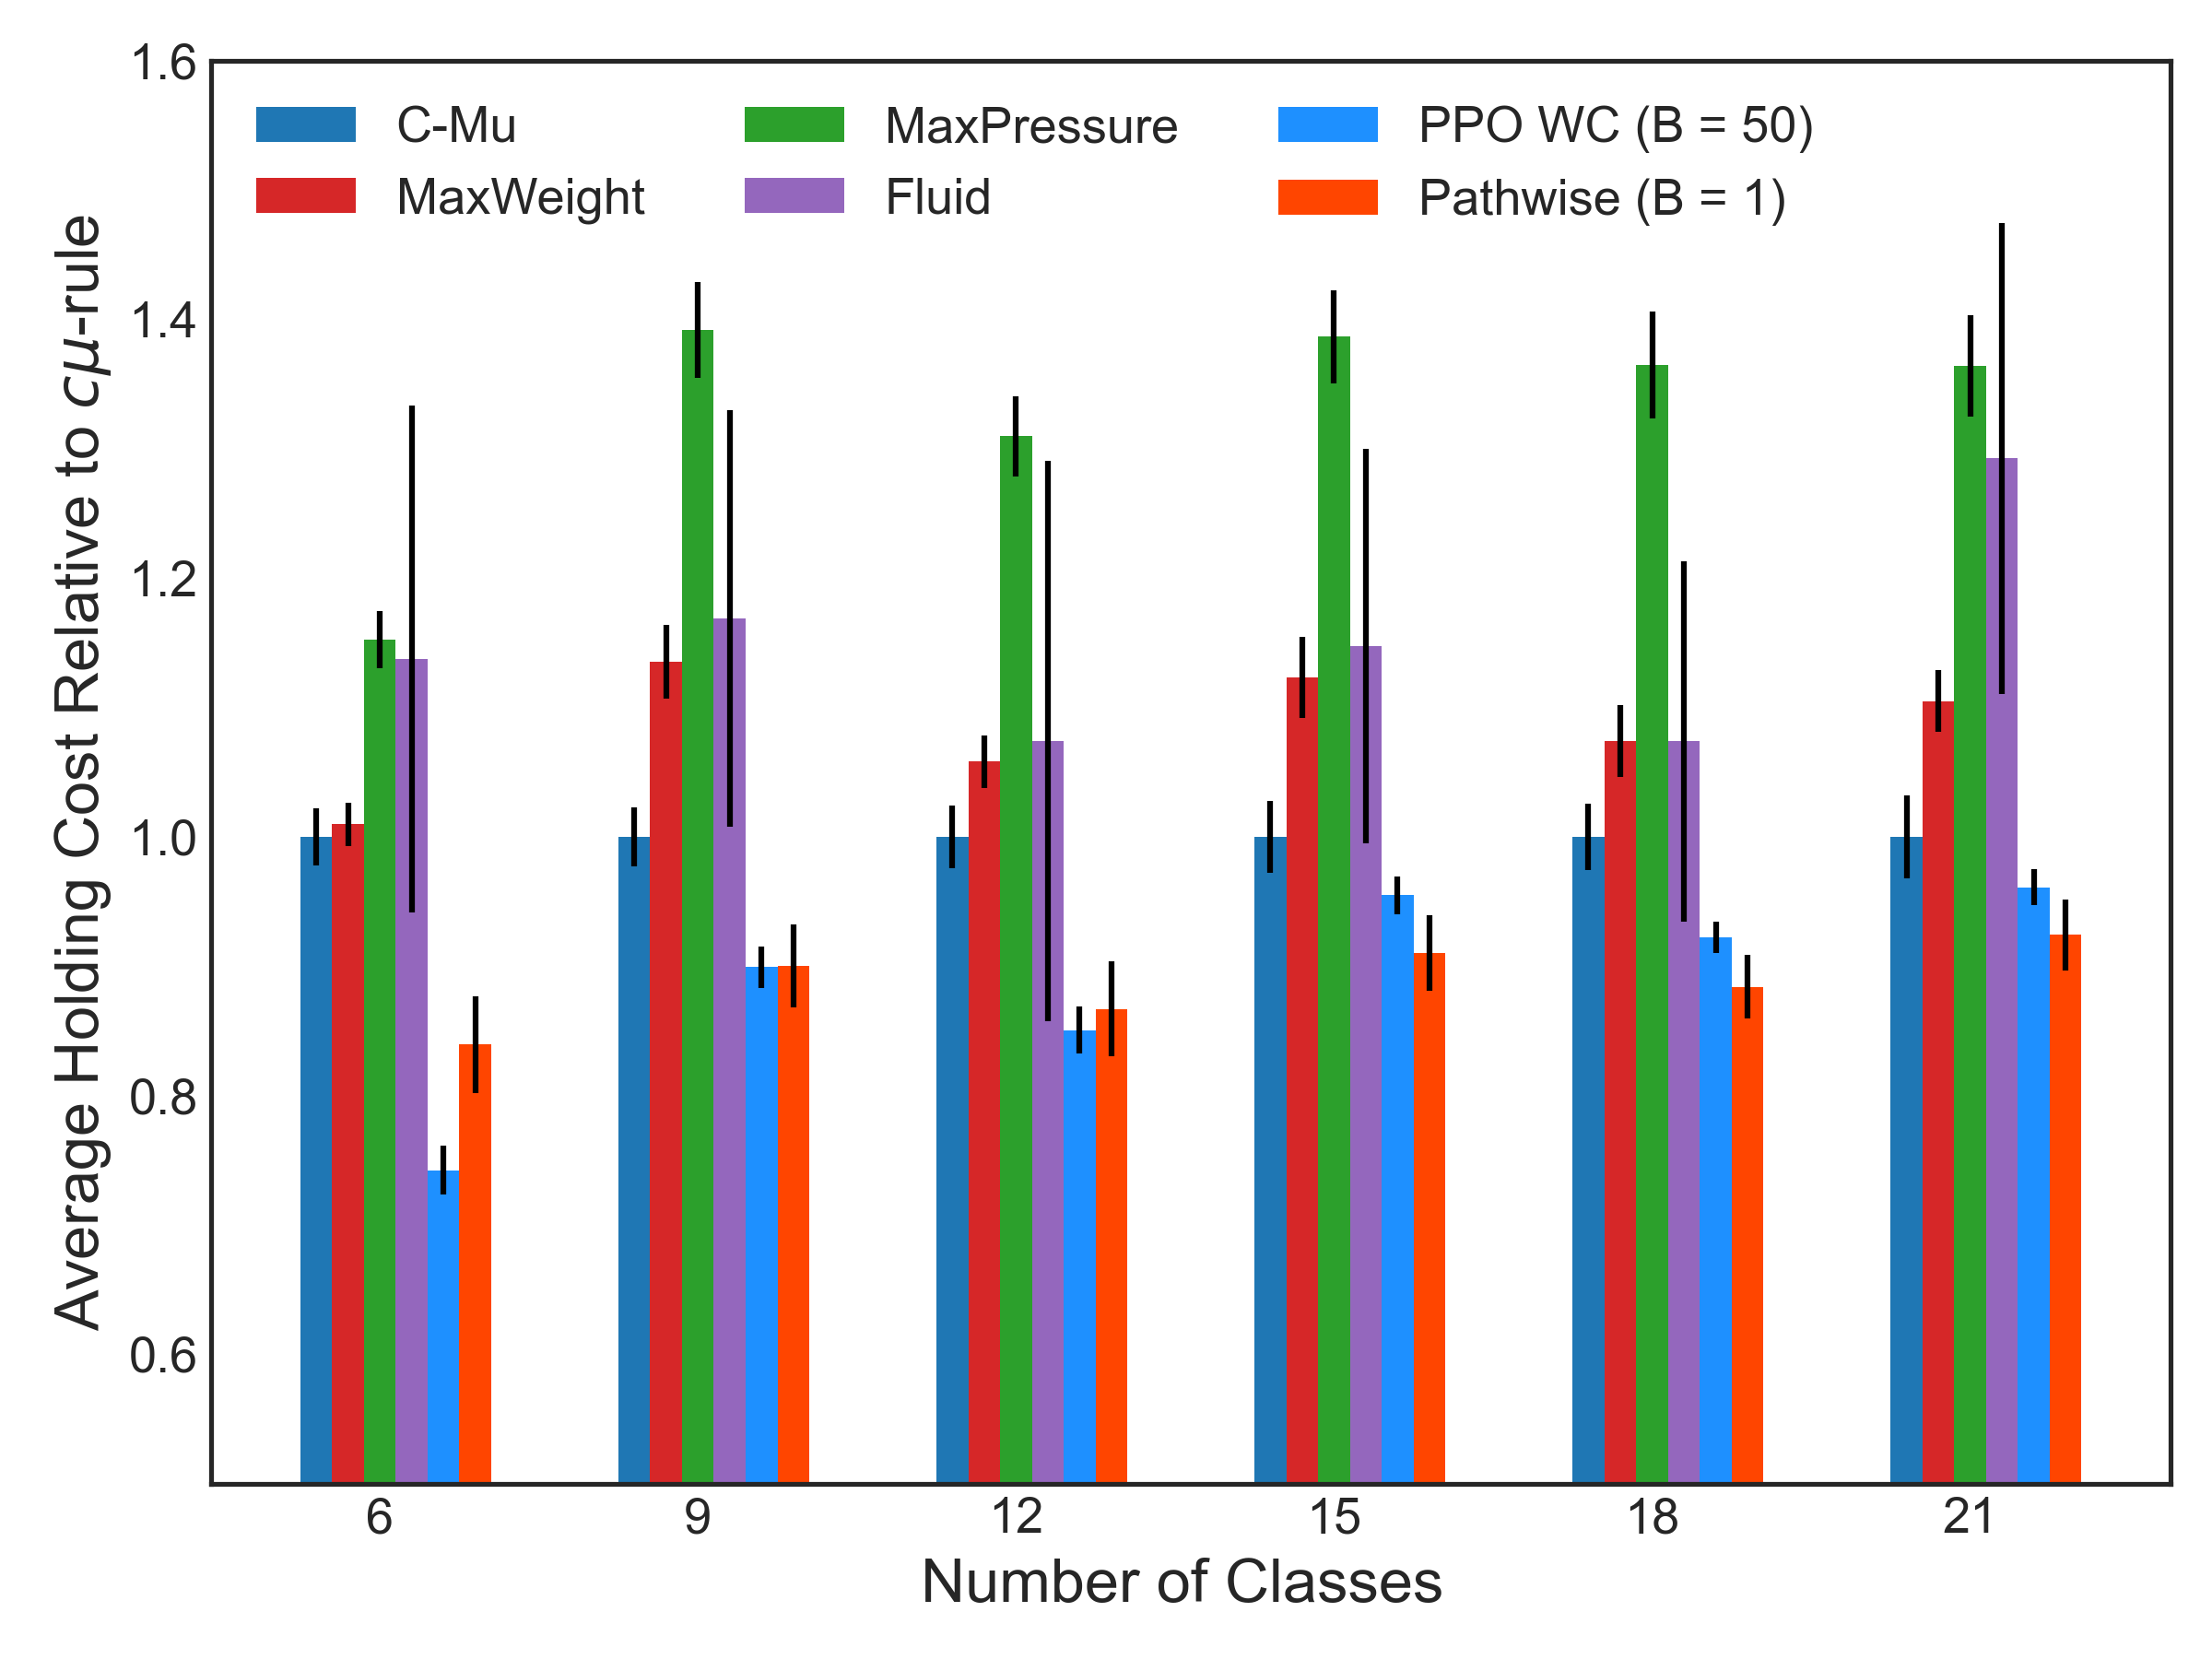
\includegraphics[height = 2.2in]{plot/results/reentrant_hyper_results.png}
% 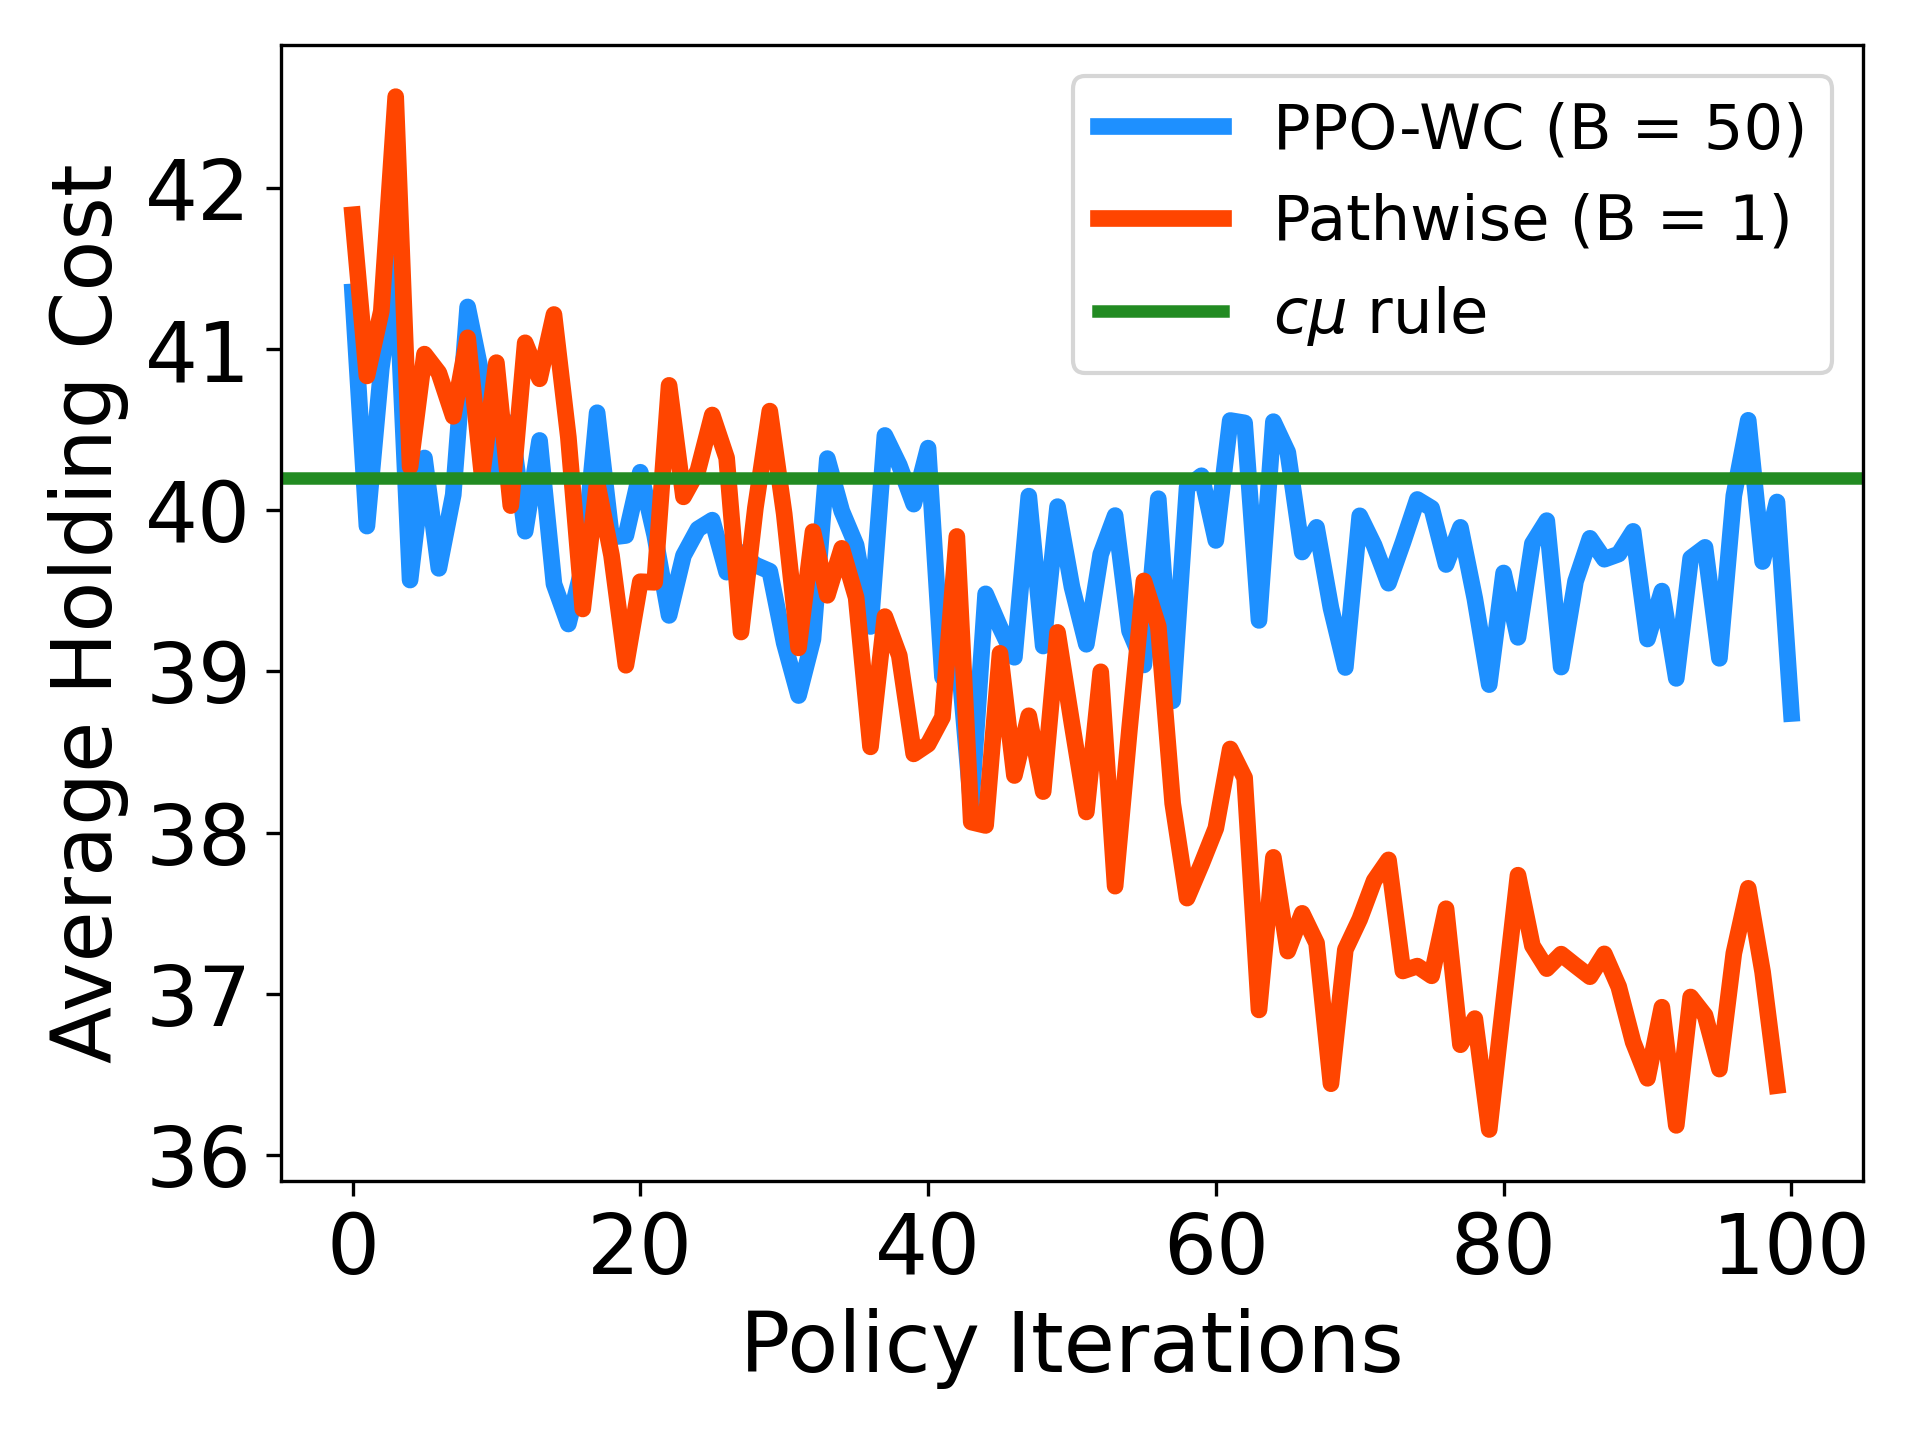
\includegraphics[height = 1.6in]{plot/results/reentrant_5.png}
% 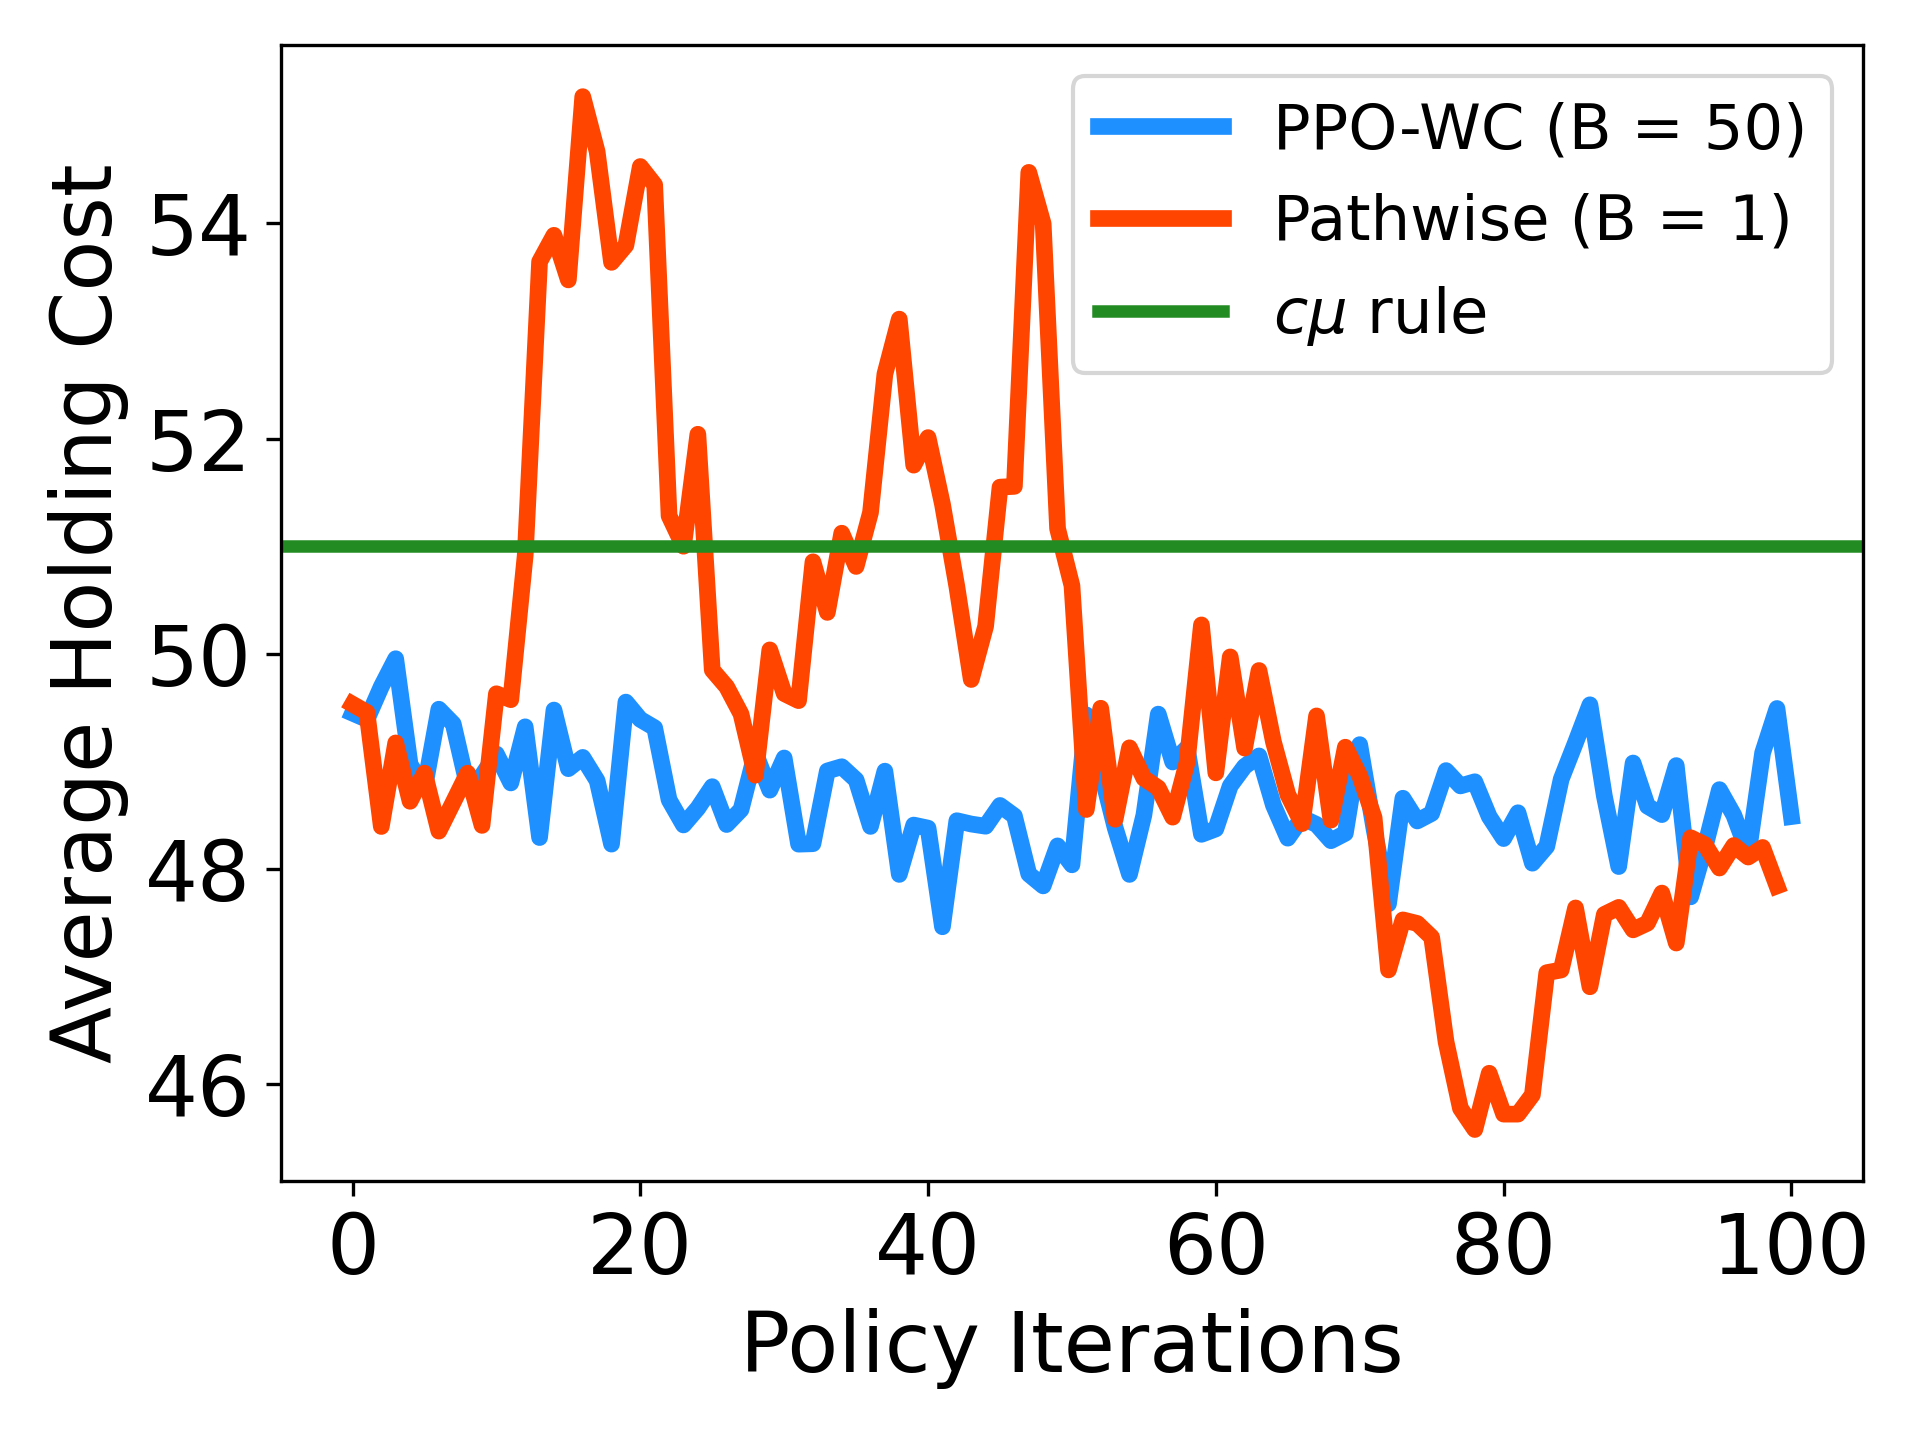
\includegraphics[height = 1.6in]{plot/results/reentrant_6.png}
% 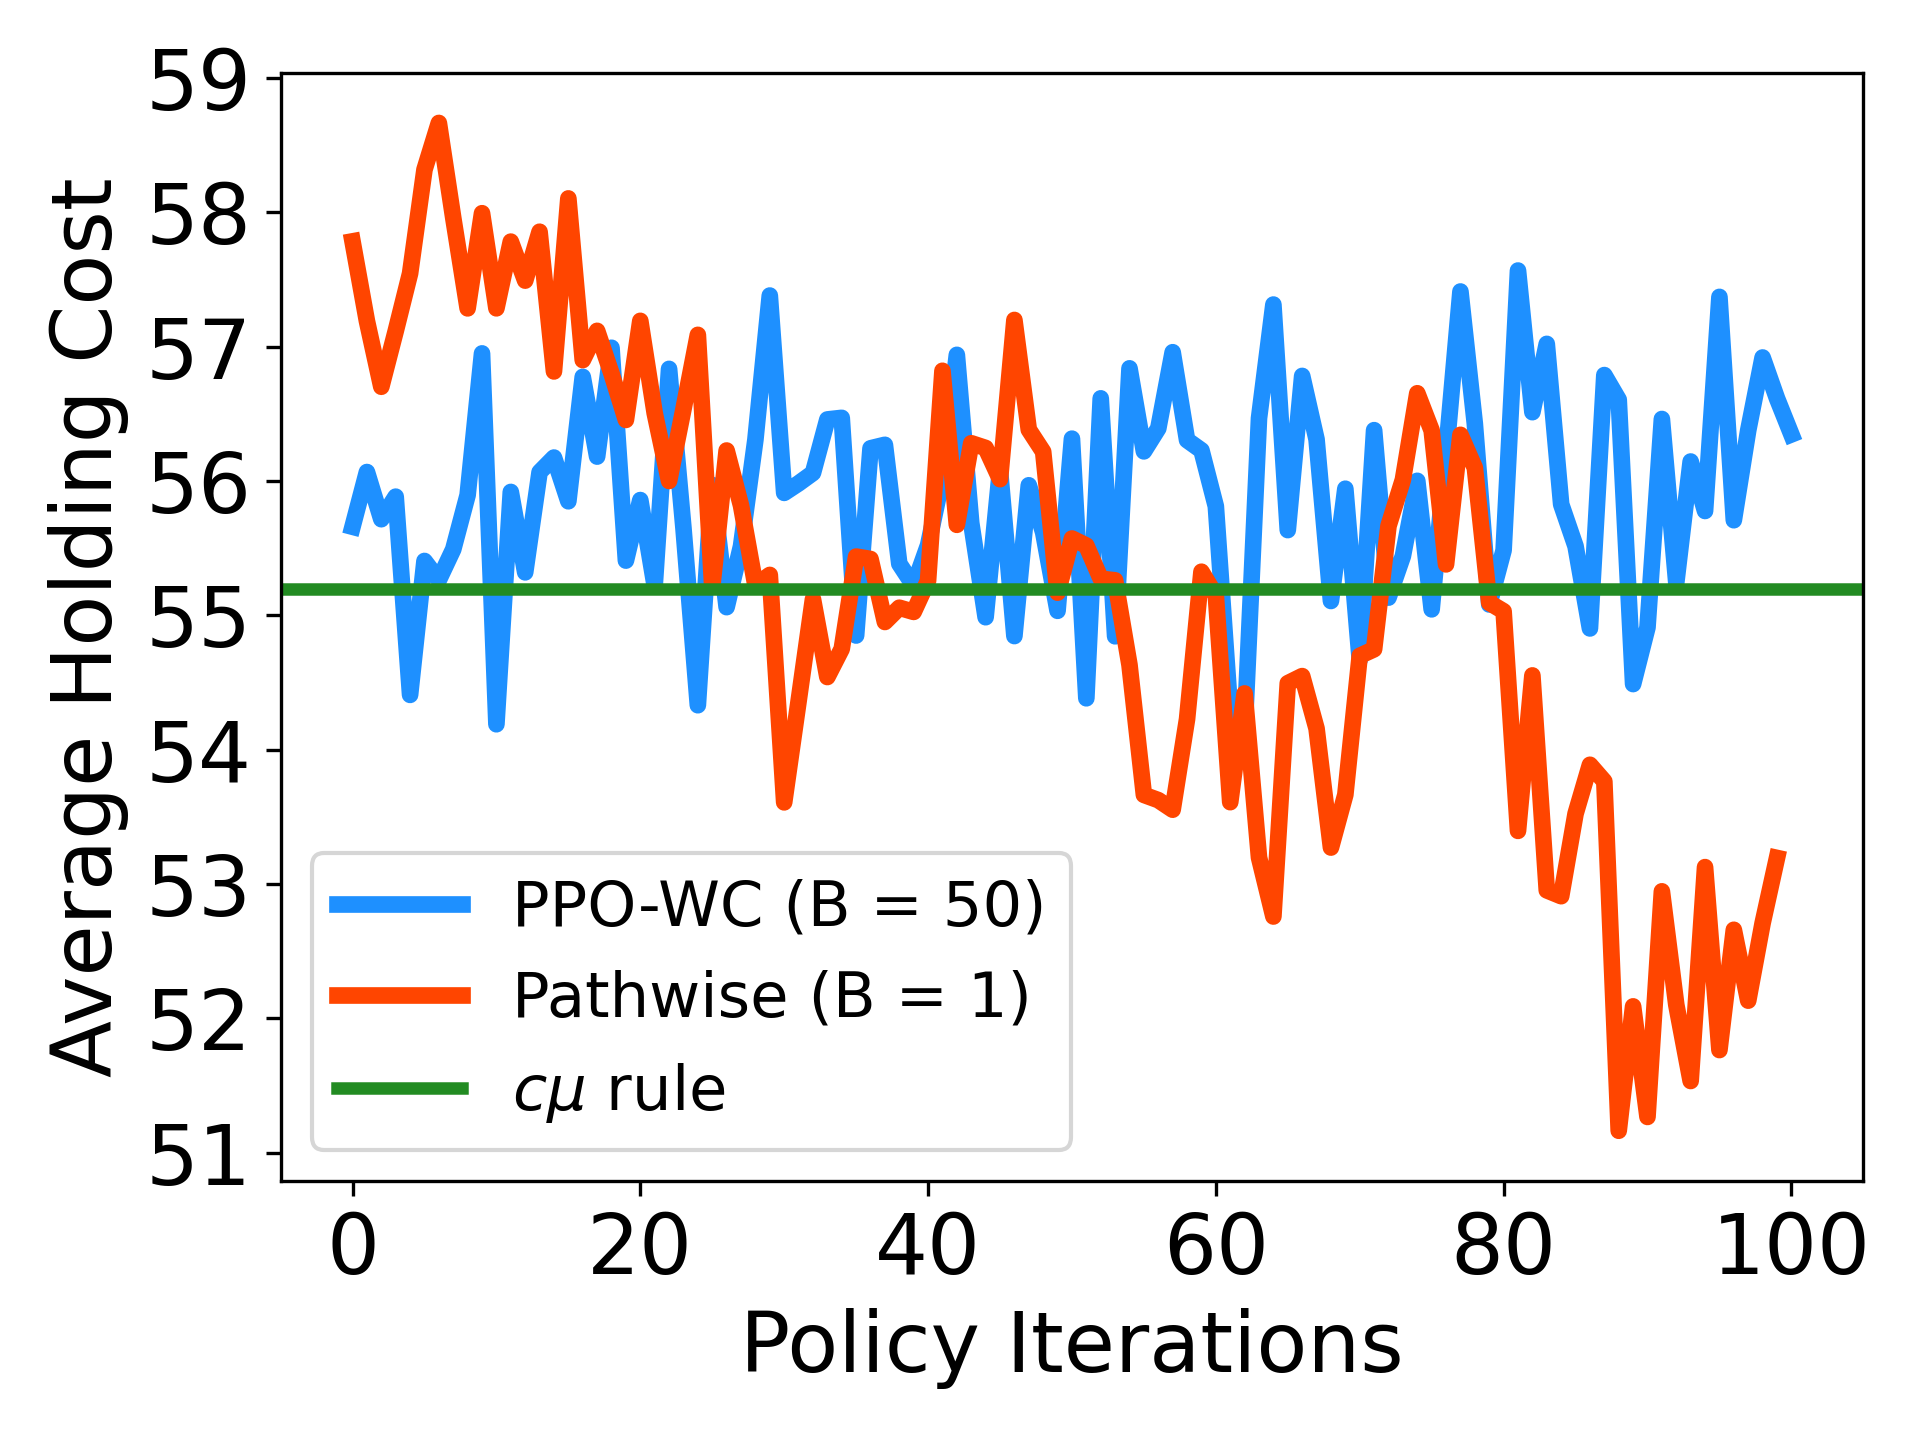
\includegraphics[height = 1.6in]{plot/results/reentrant_7.png}

% 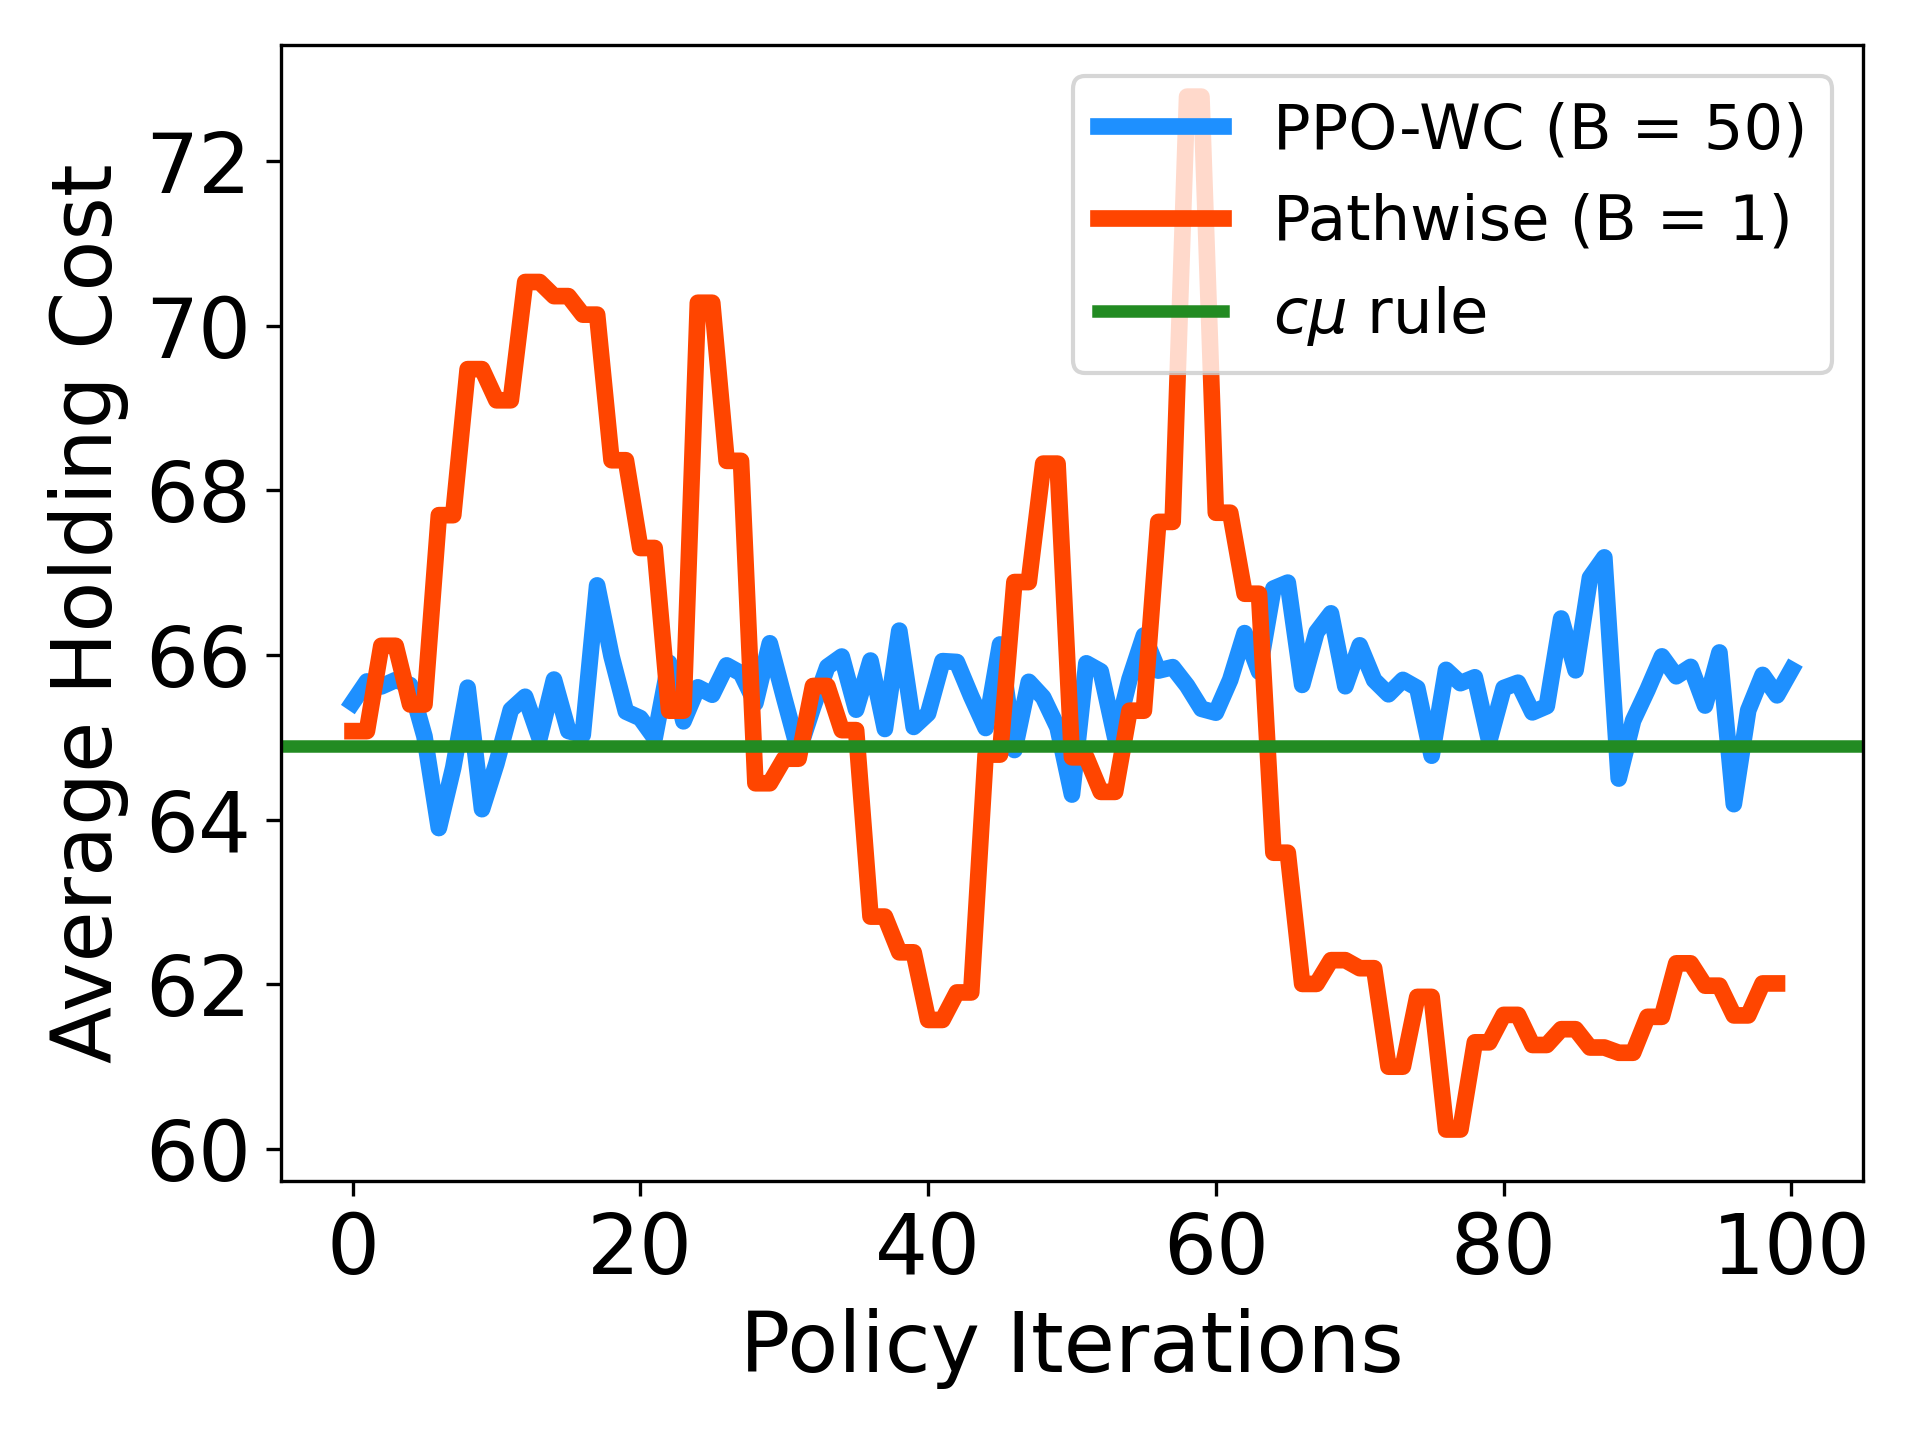
\includegraphics[height = 1.6in]{plot/results/reentrant_8.png}
% 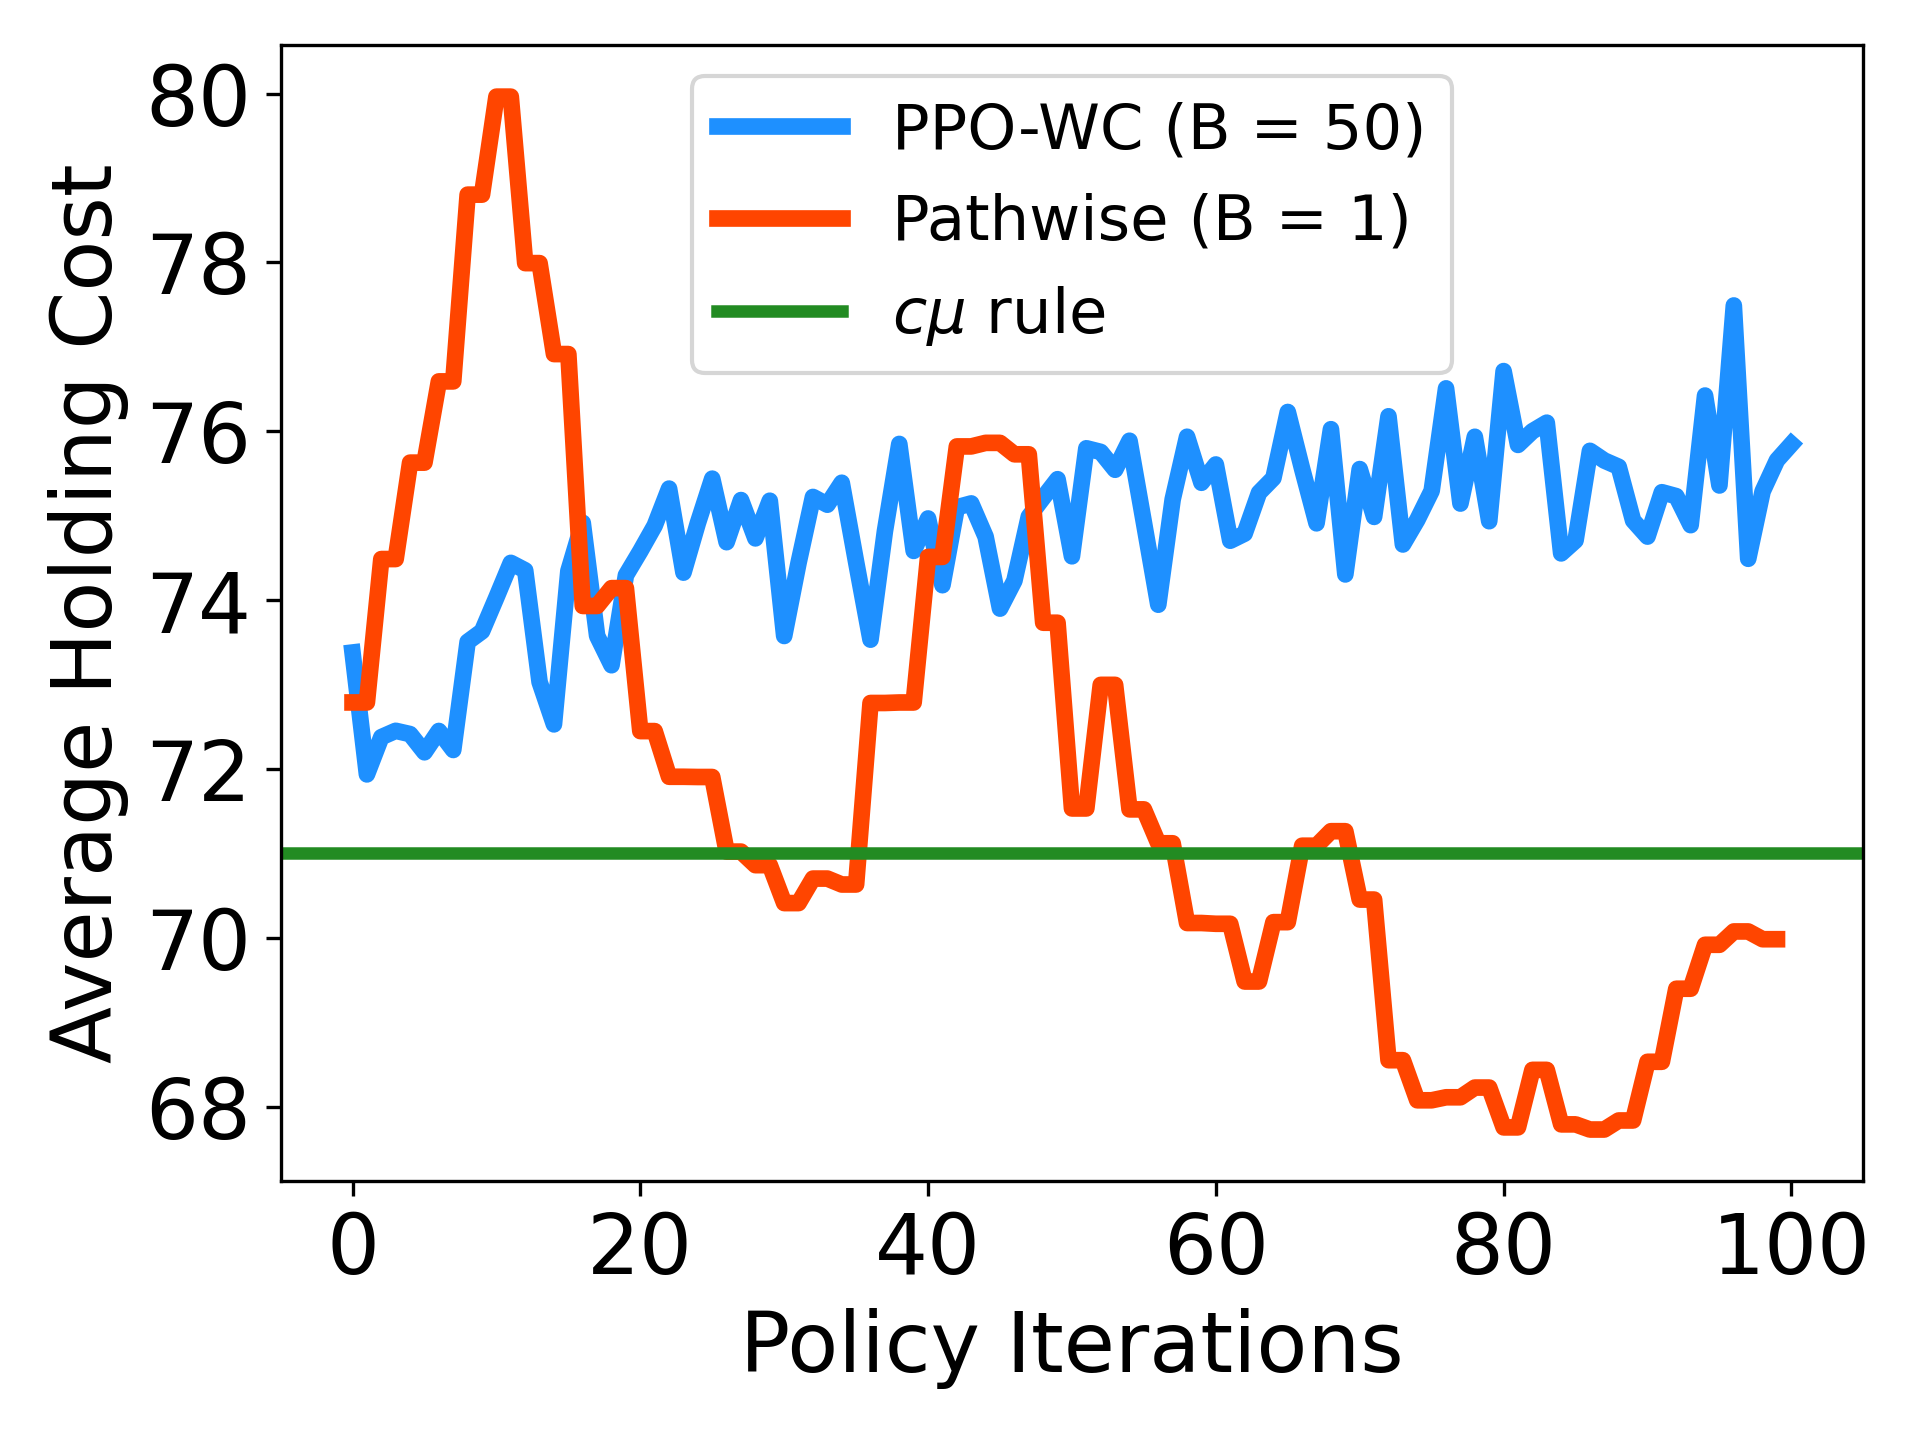
\includegraphics[height = 1.6in]{plot/results/reentrant_9.png}
% 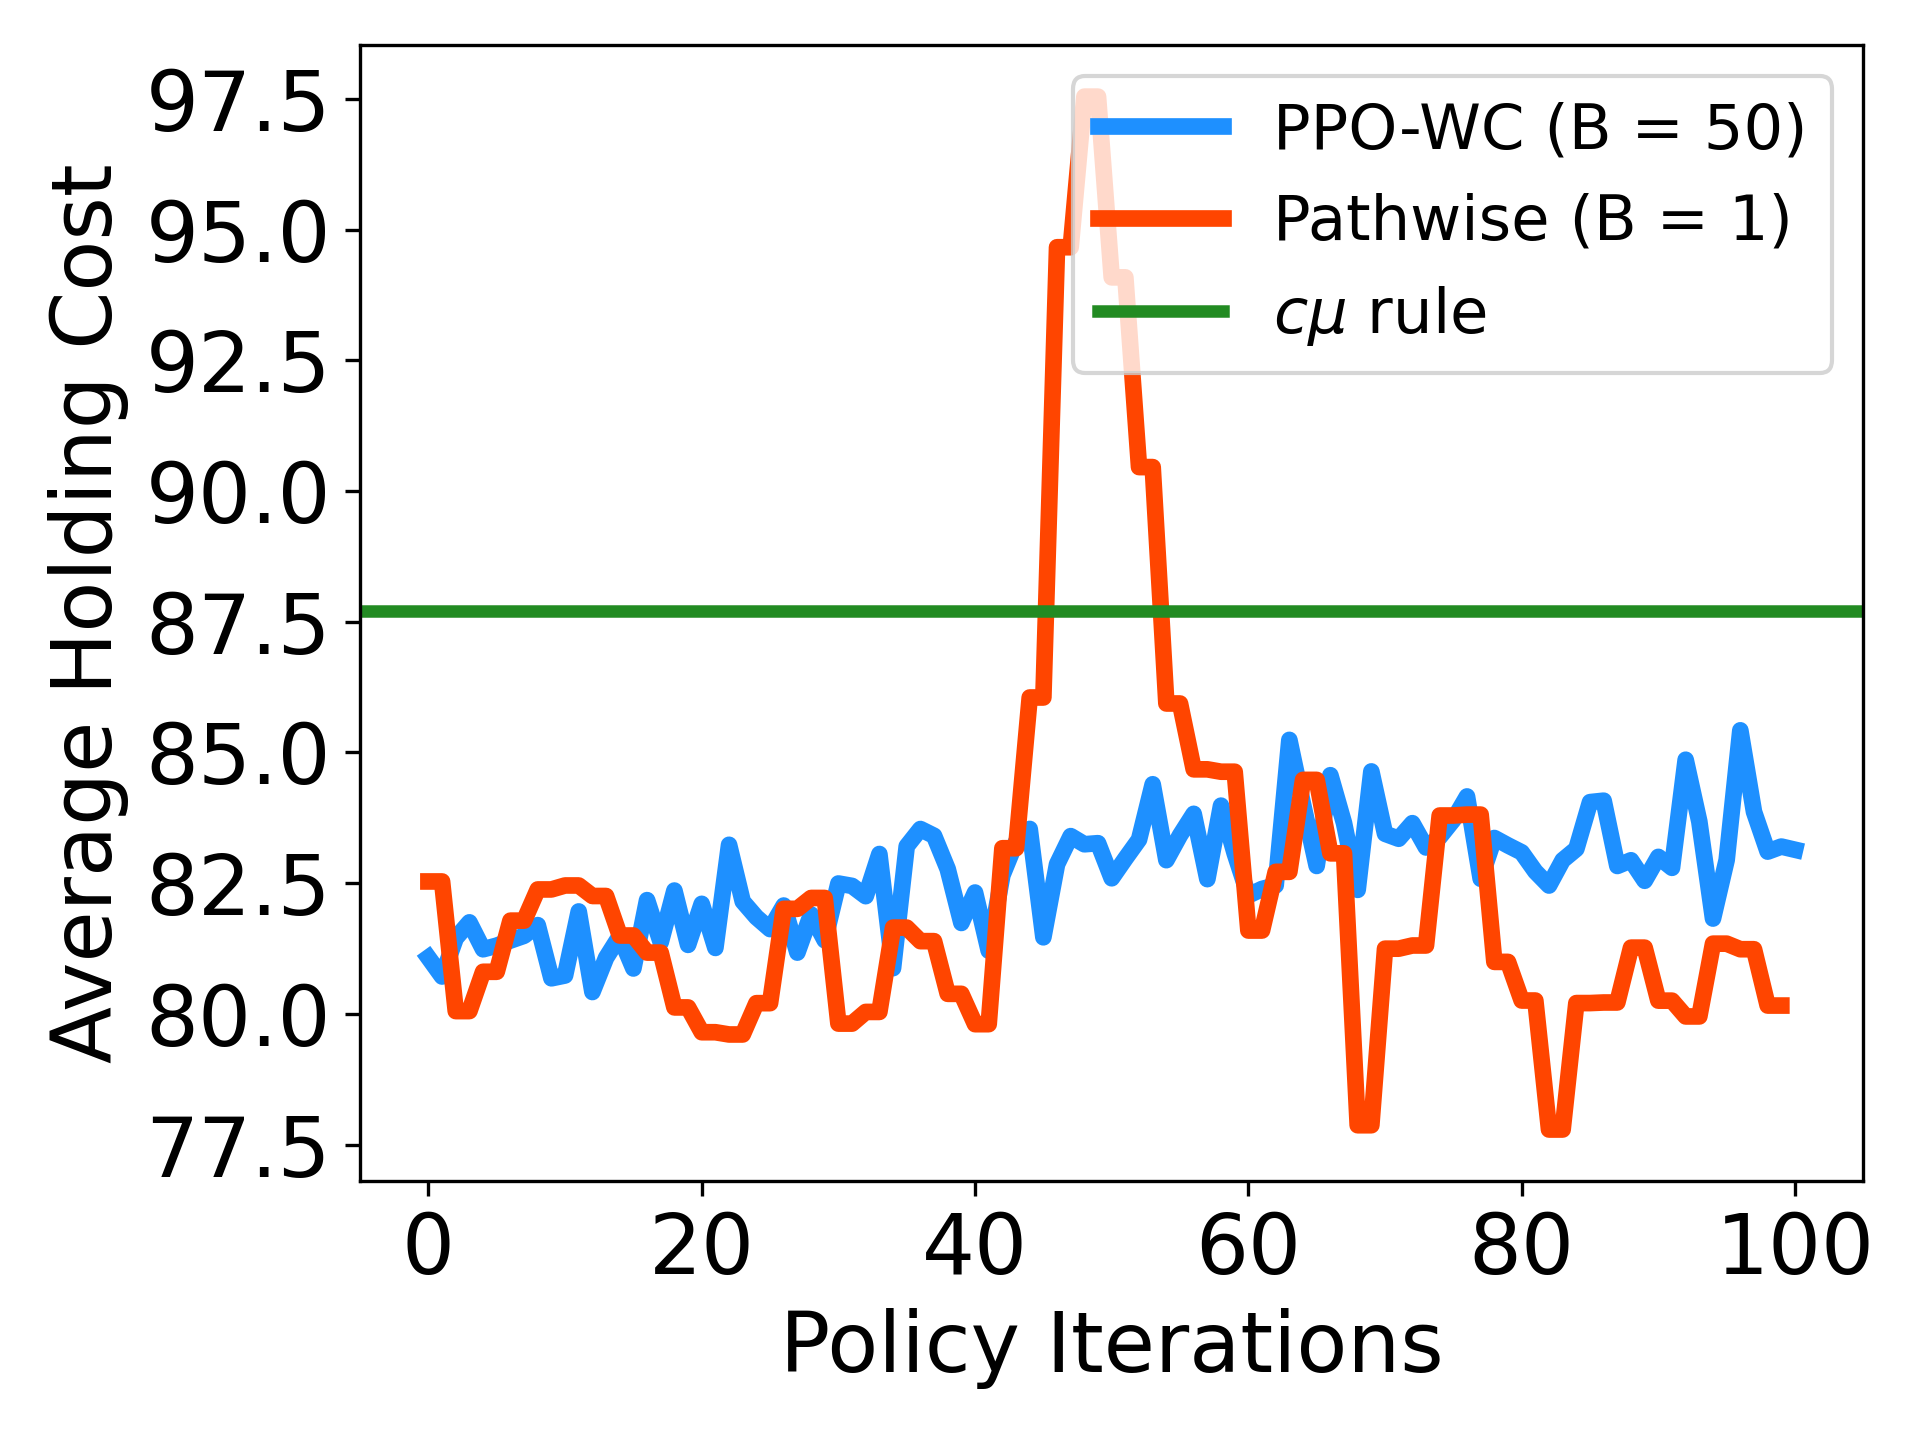
\includegraphics[height = 1.6in]{plot/results/reentrant_10.png}

    
% \caption{Comparison of policy iterations for $\ppowc$ and $\pathwise$ policy gradient (Algorithm~\ref{alg:pathwise-pg}) across several Re-entrant-1 networks. From top-left to bottom-right: Re-entrant-1 networks with 15, 18, 21, 24, 27, and 30 job classes. We run 100 policy iterations for both algorithms. $\pathwise$ uses a single trajectory for gradient estimation, whereas $\ppowc$ uses all trajectories drawn from $B = 50$ parallel actors. We plot the average holding cost of the $c\mu$-rule for comparison.}

\caption{Comparison of average holding cost of queuing control policies relative to $c\mu$-rule, including $\ppowc$ (ours) and $\pathwise$ (Algorithm~\ref{alg:pathwise-pg}). (Left) Average holding cost for the Re-entrant-1 networks with 18, 21, 24, 27, and 30 job classes. (Right) Average holding cost for the Re-entrant-1 networks with hyper-exponential inter-arrival and service times with 6, 9, 12, 14, 18, 21 job classes. $\pathwise$ outperforms $\ppowc$ for large networks in particular.}

    \label{fig:policy_iterations} 
\end{figure}
Our empirical validation goes beyond the typical settings studied in the reinforcement learning for queuing literature, and is enabled by our discrete-event simulation framework.

\begin{table*}[h!]
\centering \caption{Criss Cross}
\vspace{1em}
\label{table:criss-cross} %
\begin{tabular}{ccccccccc}
\toprule 
{\footnotesize{}Noise } & {\footnotesize{}$c\mu$ } & {\footnotesize{}MaxWeight } & {\footnotesize{}MaxPressure} & {\footnotesize{}Fluid } & {\footnotesize{}$\mathsf{PPO}$-$\mathsf{DG}$~\cite{dai2022queueing}} & {\footnotesize{}$\mathsf{PPO}$-$\mathsf{WC}$} & {\footnotesize{}$\mathsf{PATHWISE}$} &
{\footnotesize{}\% improve}\tabularnewline
\midrule 
{\footnotesize{}$\mathsf{Exp}$ } & {\footnotesize{}$17.9\pm0.3$ } & {\footnotesize{}$17.8\pm0.3$ } & {\footnotesize{}$19.0\pm0.3$ } & {\footnotesize{}$18.2\pm2.7$} & {\footnotesize{}$\mathbf{15.4\pm0.1}$ } & {\footnotesize{}$\mathbf{15.4\pm0.2}$ } & {\footnotesize{}$\mathbf{15.2\pm0.4}$} &
{\footnotesize{}$17.8\%$}
\tabularnewline
\midrule 
{\footnotesize{}$\mathsf{HyperExp}$} & {\footnotesize{}$28.4\pm0.5$ } & {\footnotesize{}$28.3\pm0.8$ } & {\footnotesize{}$28.1\pm0.8$ } &
{\footnotesize{}$27.1\pm4.7$ }& {\footnotesize{}N/A} & 
{\footnotesize{}$24.0\pm0.7$ } & 
{\footnotesize{}$\mathbf{22.5\pm0.7}$ } &
{\footnotesize{}$20.4\%$}
\tabularnewline
\bottomrule
\end{tabular}
\end{table*}

We now describe the standard queuing policies considered in this section, which can all be expressed in the form
\[
    \pi(x)=\argmax_{u\in \mathcal{U}} \sum_{i\in[m],j\in[n]} \rho_{ij}(x)u_{ij}
    \]
for some index $\rho\in \R^{m \times n}$ that differs per method.
\begin{itemize}[itemsep=0pt]
    \item $c\mu$-rule~\cite{cox1961queues}: $\rho_{ij} = h_{j}\mu_{ij}1\{x_{j} > 0 \}$. Servers prioritize queues with a higher holding cost and a larger service rate.
    %Servers are allocated to the queue with the highest $c\mu$ index
    \item MaxWeight~\cite{tassiulas1990stability, stolyar2004maxweight}: $\rho_{ij}(x) = h_{j}\mu_{ij}x_{j}$. Servers prioritize queues that are longer, with a higher holding cost, and a larger service rate.
    %Servers are allocated to the queue with the longest queue, weighted by the cost and service rate.
    \item MaxPressure~\cite{tassiulas1990stability,dai2005maximum}: $\rho_{ij}= \sum_{\ell=1}^{n}\mu_{ij}R_{j\ell}h_{\ell}x_{\ell}$. MaxPressure is a modification of MaxWeight, in the sense that it takes workload externality within the network into account through the $R_{jl}$ terms, e.g., processing a class $j$ job may generate a new class $j'$ job. 
    %Servers are allocated to the queue with longest queue, weighted by the cost and service rate.
    \item Fluid~\cite{bauerle2000asymptotic}: The scheduling policy is based on the optimal sequence of actions in the fluid relaxation, which approximates the average evolution of stochastic queue lengths by deterministic ordinary differential equations. We aim to solve the continuous-time problem
    % \begin{align*}
    % \min_{\bar{u}}\text{ } &\sum_{s=1}^{H} (h^{\top}x_{s}) \Delta t \\
    % \text{s.t. } & x_{s+1} = x_{s} + (\lambda - R(\mu \odot \bar{u}_{s}))\Delta t, \quad \forall s\in [H] \\
    % & x_{s} \geq 0, \quad \forall s\in[H] \\
    % & \bar{u}_{s} \in \mathcal{U}, \quad \forall s\in[H]
    % \end{align*}
    \begin{align*}
    \min_{\bar{u}}\text{ } & \int_{0}^{T} h^\top x(t)dt \\
    \text{s.t. } & \dot{x}(t) = \lambda - R(\mu \odot \bar{u}(t)), \quad  \forall t\in [0,T]\\
    & x(t) \geq 0, \quad \forall t\in [0,T] \\
    & \bar{u}(t) \in \overline{\mathcal{U}}, \quad \forall t\in [0,T].
    \end{align*}
    For tractability, we discretize the problem with time increment $\Delta t > 0$ and horizon $H=T/\Delta t$, and solve as a linear program.
    We then set $u_{k} = \overline{u}(t_{k})$. The linear program is re-solved periodically to improve fidelity with the original stochastic dynamics.
\end{itemize}
We next describe the deep reinforcement learning methods considered in this section:
\begin{itemize}[itemsep=0pt]
    \item $\ppo$-$\mathsf{DG}$~\cite{dai2022queueing}: $\ppo$ is a standard model-free policy gradient method~\cite{schulman2017proximal, huang2022implementation}. ~\citet{dai2022queueing} implement $\ppo$ for multi-class queuing networks and show that the policies obtained outperform several standard queuing policies. 
    Their implementation includes an initial behavioral cloning for stability and a carefully designed variance-reducing policy gradient estimation. We report the results from their paper, although in our experiments we include several problem instances not evaluated in their work.
    \item $\ppo$-$\mathsf{WC}$ (ours): Given the empirical success of $\ppo$ with the work-conserving $\softmax$, we use this algorithm as the main RL benchmark. For this policy, we use the same neural network architecture, hyper-parameters, and variance reduction methods as $\ppo$-$\mathsf{DG}$ ~\cite{dai2022queueing}.
    \item $\pathwise$ policy gradient (Algorithm~\ref{alg:pathwise-pg}): Trains a neural network policy with work-conserving $\softmax$ using the $\pathwise$ policy  gradient estimator. We use an inverse temperature of $\beta = 10$ for all experiments in this section.
\end{itemize}
While value-based methods have also been considered for queuing network control~\cite{liu2022rl,wei2024sample}, our focus in this work is on benchmarking policy gradient algorithms. 

For the reinforcement learning policies, we train each method over $100$ episodes, each consisting of $N = 50,000$ environment steps. Following~\citet{dai2022queueing}'s implementation, $\ppo$-$\mathsf{WC}$ was trained with $B = 50$ actors, while $\pathwise$ was trained only with $B = 1$ actor, which means that $\ppo$-based methods used 50x more trajectories than $\pathwise$. See Appendix~\ref{sec:training-details} for more details on the training process.






To evaluate each scheduling policy, we run $100$ parallel episodes starting from empty queues $x_{0} = \mathbf{0}_{n}$ with a long horizon $N$ to estimate the long-run average holding cost (typically $N =200,000$ steps). As in previous works (e.g.~\cite{dai2022queueing, bertsimas2014robust}), we consider holding costs $h = \ones_{n}$ in which case the holding cost is equivalent to the total queue length. To reiterate, for each policy $\pi$ we estimate the following quantity 
\begin{equation}
    J_{N}(\pi) = 
  \E \left[\frac{1}{t_{N}}\sum_{k=0}^{N-1} (\ones_{n}^{\top}x_{k})\tau^{*}_{k+1} \right]
=  \E \left[\frac{1}{t_{N}} \int^{t_{N}}_{0} \sum_{i=1}^{n} x_{i}(t)dt \right]
\end{equation}
where $t_{N}$ is the time of the $N$th event. We measure the standard deviation across the 100 episodes to form 95\% confidence intervals. For the reinforcement learning policies, we report the average holding cost for the best policy encountered during training.


\vspace{1em}
\begin{table*}[h!]
\centering
 \caption{Re-entrant-1 ($\mathsf{Exp}$)}%
\begin{tabular}{ccccccccc}
\toprule 
{\footnotesize{}Classes} & {\footnotesize{}$c\mu$ } & {\footnotesize{}MaxWeight } & {\footnotesize{}MaxPressure} & {\footnotesize{}Fluid } & {\footnotesize{}$\mathsf{PPO}$-$\mathsf{DG}$~\cite{dai2022queueing} } & {\footnotesize{}$\ppowc$} & {\footnotesize{}$\mathsf{PATHWISE}$} & {\footnotesize{}\% improve}\tabularnewline
\midrule 
{\footnotesize{}6} & {\footnotesize{}$17.4\pm0.4$ } & {\footnotesize{}$17.5\pm0.4$ } & {\footnotesize{}$18.8\pm0.5$ } & {\footnotesize{}$16.8\pm4.3$} & {\footnotesize{}$14.1\pm0.2$ } & {\footnotesize{}$\mathbf{13.6\pm0.4}$ } & {\footnotesize{}$14.9\pm0.5$ } & {\footnotesize{}14.3\%}\tabularnewline
\midrule 
{\footnotesize{}9} & {\footnotesize{}$23.3\pm0.6$ } & {\footnotesize{}$26.1\pm0.5$ } & {\footnotesize{}$24.2\pm0.6$ } & {\footnotesize{}$27.7\pm4.4$} & {\footnotesize{}$23.3\pm0.3$ } & {\footnotesize{}${\bf 22.6\pm0.4}$ } & {\footnotesize{}${\bf 22.0\pm0.6}$ } & {\footnotesize{}4.3\%}\tabularnewline
\midrule 
{\footnotesize{}12 } & {\footnotesize{}$33.0\pm0.8$ } & {\footnotesize{}$34.0\pm1.0$ } & {\footnotesize{}$35.1\pm0.9$ } & {\footnotesize{}$40.6\pm4.8$} & {\footnotesize{}$32.2\pm0.6$ } & {\footnotesize{}$\mathbf{29.7\pm0.4}$ } & {\footnotesize{}$\mathbf{30.7\pm0.7}$ } & {\footnotesize{}7.0\%}\tabularnewline
\midrule 
{\footnotesize{}15 } & {\footnotesize{}$40.2\pm1.3$ } & {\footnotesize{}$43.6\pm1.1$ } & {\footnotesize{}$42.2\pm1.3$ } & {\footnotesize{}$49.8\pm5.1$} & {\footnotesize{}$39.3\pm0.6$ } & {\footnotesize{}$38.7\pm0.4$ } & {\footnotesize{}$\mathbf{36.2\pm0.8}$ } & {\footnotesize{}9.9\%}\tabularnewline
\midrule 
{\footnotesize{}18 } & {\footnotesize{}$ 48.5\pm1.0$ } & {\footnotesize{}$51.0\pm1.4$ } & {\footnotesize{}$52.4\pm1.6$ } & {\footnotesize{}$54.5\pm4.2$} & {\footnotesize{}$51.4\pm1.0$ } & {\footnotesize{}$47.5\pm0.5$ } & {\footnotesize{}$\mathbf{45.7\pm0.7}$ } & {\footnotesize{}$5.7\%$}\tabularnewline
\midrule 
{\footnotesize{}21 } & {\footnotesize{}$55.2\pm1.1$ } & {\footnotesize{}$59.5\pm1.6$ } & {\footnotesize{}$56.0\pm1.6$} & {\footnotesize{}$63.7\pm6.7$} & {\footnotesize{}$55.1\pm1.8$} & {\footnotesize{}$56.3\pm0.8$ } & {\footnotesize{}$\mathbf{52.8\pm1.2}$ } & {\footnotesize{}4.3\%}\tabularnewline
\midrule 
{\footnotesize{}24 } & {\footnotesize{}$64.9\pm1.4$ } & {\footnotesize{}$69.4\pm1.6$ } & {\footnotesize{}$66.6\pm2.2$ } & {\footnotesize{}$74.0\pm6.7$} & {\footnotesize{}N/A} & {\footnotesize{}$65.8\pm0.6$ } & {\footnotesize{}$\mathbf{60.2\pm0.9}$ } & {\footnotesize{}6.2\%}\tabularnewline
\midrule 
{\footnotesize{}27 } & {\footnotesize{}$71.1\pm1.5$ } & {\footnotesize{}$77.7\pm1.9$ } & {\footnotesize{}$72.0\pm2.5$ } & {\footnotesize{}$83.1\pm7.1$} & {\footnotesize{}N/A} & {\footnotesize{}$75.8\pm0.7$ } & {\footnotesize{}$\mathbf{67.7\pm1.3}$ } & {\footnotesize{}3.0\%}\tabularnewline
\midrule 
{\footnotesize{}30 } & {\footnotesize{}$87.7\pm2.5$ } & {\footnotesize{}$84.5\pm2.1$ } & {\footnotesize{}$106.8\pm2.5$ } & {\footnotesize{}$93.6\pm8.0$} & {\footnotesize{}N/A} & {\footnotesize{}$83.1\pm0.7$ } & {\footnotesize{}$\mathbf{77.8\pm1.3}$ } & {\footnotesize{}7.9\%}\tabularnewline
\bottomrule
\end{tabular}
\vspace{1em}
 \caption{Re-entrant-1 ($\mathsf{HyperExp}$)}
\begin{tabular}{cccccccc}
\toprule 
{\footnotesize{}Classes} & {\footnotesize{}$c\mu$ } & {\footnotesize{}MaxWeight } & {\footnotesize{}MaxPressure} & {\footnotesize{}Fluid } & {\footnotesize{}$\mathsf{PPO}$-$\mathsf{WC}$} & {\footnotesize{}$\mathsf{PATHWISE}$} & {\footnotesize{}\% improve}\tabularnewline
\midrule 
{\footnotesize{}6} & {\footnotesize{}$37.8\pm1.3$} & {\footnotesize{}$39.2\pm1.2$} & {\footnotesize{}$43.8\pm1.8$} & {\footnotesize{}$43.6\pm7.5$} & {\footnotesize{}$\mathbf{29.9\pm0.7}$} & {\footnotesize{}$32.2\pm1.4$ } & {\footnotesize{}6.9\%}\tabularnewline
\midrule 
{\footnotesize{}9} & {\footnotesize{}$50.2\pm1.9$} & {\footnotesize{}$55.5\pm2.2$} & {\footnotesize{}$68.7\pm2.7$} & {\footnotesize{}$59.2\pm8.2$} & {\footnotesize{}$\mathbf{47.5\pm0.8}$} & {\footnotesize{}$\mathbf{45.6\pm1.6}$ } & {\footnotesize{}9.2\%}\tabularnewline
\midrule 
{\footnotesize{}12 } & {\footnotesize{}$70.0\pm2.5$} & {\footnotesize{}$72.3\pm2.8$} & {\footnotesize{}$89.4\pm3.6$} & {\footnotesize{}$75.6\pm15.3$} & {\footnotesize{}$64.4\pm1.2$} & {\footnotesize{}$\mathbf{61.1\pm2.5}$ } & {\footnotesize{}12.7\%}\tabularnewline
\midrule 
{\footnotesize{}15 } & {\footnotesize{}$81.7\pm4.0$} & {\footnotesize{}$91.0\pm3.7$} & {\footnotesize{}$112.0\pm4.9$} & {\footnotesize{}$97.0\pm12.9$} & {\footnotesize{}$81.8\pm1.1$} & {\footnotesize{}${\bf 76.9\pm2.5}$ } & {\footnotesize{}5.9\%}\tabularnewline
\midrule 
{\footnotesize{}18 } & {\footnotesize{}$101.1\pm4.7$} & {\footnotesize{}$103.9\pm3.9$} & {\footnotesize{}$126.7\pm6.2$} & {\footnotesize{}$111.2\pm14.4$} & {\footnotesize{}$99.8\pm1.5$} & {\footnotesize{}${\bf 91.5\pm2.5}$ } & {\footnotesize{}9.4\%}\tabularnewline
\midrule 
{\footnotesize{}21 } & {\footnotesize{}$116.3\pm4.6$} & {\footnotesize{}$123.3\pm3.9$} & {\footnotesize{}$152.3\pm6.6$} & {\footnotesize{}$151.0\pm21.3$} & {\footnotesize{}$118.2\pm2.0$} & {\footnotesize{}${\bf 108.0\pm3.2}$ } & {\footnotesize{}7.2\%}\tabularnewline
\bottomrule
\end{tabular}
\end{table*}

Tables 1-5 display the results of our benchmarking across the problem instances discussed before. The column `\% improve' records the relative reduction in holding cost achieved by $\pathwise$ over the best standard queuing policy (either $c\mu$, MaxWeight, MaxPressure, or Fluid). Our main observations on the relative performance of the standard policies and policies obtained from reinforcement learning methods are summarized as follows.
\begin{itemize}[itemsep=0pt]
    \item {\bf $\ppowc$ is a strong reinforcement-learning benchmark.} $\ppo$ with our proposed work-conserving $\softmax$ is able to efficiently find policies that outperform standard policies across all problem instances, as well as the $\ppo$ featured in~\cite{dai2022queueing} (under the same policy network and hyper-parameters). This illustrates that simply ensuring work-conservation is a powerful inductive bias that delivers stability.
    \item {\bf $\pathwise$ policy gradient outperforms $\ppowc$ in larger networks, using 50x less data}. We observe that $\ppowc$ and $\pathwise$ achieve similar performances when the number of classes is small. However, when the number of job classes gets larger, $\pathwise$ consistently outperforms $\ppowc$, as seen in Figure~\ref{fig:policy_iterations}. This is likely due to the 
    %For smaller networks, the performance is equivalent. This is a practical demonstration of the improvement in 
    sample efficiency gained by the $\pathwise$ gradient, enabling the algorithm to find better policies with less data.
    \item {\bf $\pathwise$ achieves large performance gains over  $\ppowc$ for higher-variance problem instances, using 50x less data}. We observe that for the Re-entrant-1 networks with hyper-exponential noise, the reduction of holding cost of $\pathwise$ relative to $\ppowc$ is often equivalent or even larger than the cost reduction of $\ppowc$ relative to the $c\mu$-rule. This illustrates that even among optimized RL policies, there can be significant performance differences for difficult problem instances, and the sample efficiency of $\pathwise$ is particularly useful in noisier environments.
    \item {\bf While standard queuing methods work well, RL methods meaningfully improve performance in hard instances.} We observe in the `\% improve' column that $\pathwise$ achieves a 3-20\% improvement over the best standard queuing policy in each setting.
\end{itemize}



Altogether, these results illustrate that policy gradient with $\pathwise$ gradient estimator and work-conserving $\softmax$ policy architecture can learn effective queuing network control policies with substantially less data than model-free policy gradient algorithms for large networks with high-variance event times, mirroring real-world systems. 
In particular, the improved sample efficiency of the $\pathwise$ gradient estimator and the stability brought by work-conserving $\softmax$ policy architecture are the keys to enabling learning in large-scale systems with realistic data requirements.



\begin{table}[h!]
\centering
 \caption{Re-entrant-2 ($\mathsf{Exp}$)}%
\begin{tabular}{cccccccc}
\toprule 
{\footnotesize{}Classes} & {\footnotesize{}$c\mu$ } & {\footnotesize{}MaxWeight } & {\footnotesize{}MaxPressure} & {\footnotesize{}Fluid } & {\footnotesize{}$\mathsf{PPO}$-$\mathsf{WC}$ } & {\footnotesize{}$\mathsf{PATHWISE}$} & {\footnotesize{}\% improve}\tabularnewline
\midrule 
{\footnotesize{}6} & {\footnotesize{}$18.8\pm0.5$} & {\footnotesize{}$17.4\pm0.4$} & {\footnotesize{}$24.5\pm0.7$} & {\footnotesize{}$18.6\pm2.8$} & {\footnotesize{}$\mathbf{13.7\pm0.2}$} & {\footnotesize{}$14.7\pm0.6$} & {\footnotesize{}21.9\%}\tabularnewline
\midrule 
{\footnotesize{}9} & {\footnotesize{}$24.2\pm0.6$} & {\footnotesize{}$25.8\pm0.7$} & {\footnotesize{}$31.5\pm1.0$} & {\footnotesize{}$26.7\pm3.7$} & {\footnotesize{}$\mathbf{22.1\pm0.3}$} & {\footnotesize{}$\mathbf{21.6\pm0.6}$} & {\footnotesize{}10.7\%}\tabularnewline
\midrule 
{\footnotesize{}12 } & {\footnotesize{}$35.1\pm0.9$} & {\footnotesize{}$34.0\pm1.1$} & {\footnotesize{}$40.3\pm1.4$} & {\footnotesize{}$35.7\pm4.6$} & {\footnotesize{}$\mathbf{29.9\pm0.5}$} & {\footnotesize{}$\mathbf{29.8\pm0.7}$} & {\footnotesize{}15.1\%}\tabularnewline
\midrule 
{\footnotesize{}15 } & {\footnotesize{}$44.8\pm1.3$} & {\footnotesize{}$43.8\pm1.5$} & {\footnotesize{}$50.1\pm1.6$} & {\footnotesize{}$44.0\pm5.3$} & {\footnotesize{}$\mathbf{38.0\pm0.5}$} & {\footnotesize{}$\mathbf{36.2\pm1.0}$} & {\footnotesize{}19.2\%}\tabularnewline
\midrule 
{\footnotesize{}18 } & {\footnotesize{}$52.4\pm1.6$} & {\footnotesize{}$48.7\pm1.3$} & {\footnotesize{}$58.2\pm2.1$} & {\footnotesize{}$55.2\pm5.8$} & {\footnotesize{}$\mathbf{46.8\pm0.5}$} & {\footnotesize{}$\mathbf{45.6\pm0.8}$} & {\footnotesize{}13.0\%}\tabularnewline
\midrule 
{\footnotesize{}21 } & {\footnotesize{}$56.0\pm1.6$} & {\footnotesize{}$57.5\pm1.8$} & {\footnotesize{}$71.3\pm2.9$} & {\footnotesize{}$62.2\pm7.5$} & {\footnotesize{}$55.5\pm0.6$} & {\footnotesize{}$\mathbf{51.4\pm1.1}$} & {\footnotesize{}8.2\%}\tabularnewline
\midrule 
{\footnotesize{}24 } & {\footnotesize{}$66.6\pm2.2$} & {\footnotesize{}$69.0\pm1.7$} & {\footnotesize{}$76.0\pm3.0$} & {\footnotesize{}$70.8\pm7.7$} & {\footnotesize{}$63.2\pm0.7$} & {\footnotesize{}$\mathbf{59.8\pm1.4}$} & {\footnotesize{}10.2\%}\tabularnewline
\midrule 
{\footnotesize{}27 } & {\footnotesize{}$72.0\pm2.5$} & {\footnotesize{}$75.9\pm2.1$} & {\footnotesize{}$84.9\pm3.2$} & {\footnotesize{}$82.9\pm9.6$} & {\footnotesize{}${\bf 70.3\pm0.9}$} & {\footnotesize{}$\mathbf{68.4\pm1.6}$} & {\footnotesize{}5.0\%}\tabularnewline
\midrule 
{\footnotesize{}30 } & {\footnotesize{}$80.6\pm2.7$} & {\footnotesize{}$83.8\pm1.9$} & {\footnotesize{}$90.6\pm3.2$} & {\footnotesize{}$91.2\pm11.3$} & {\footnotesize{}$80.4\pm0.8$} & {\footnotesize{}$\mathbf{75.5\pm1.8}$} & {\footnotesize{}6.3\%}\tabularnewline
\bottomrule
\end{tabular}

 \caption{Re-entrant-2 ($\mathsf{HyperExp}$)}

\begin{tabular}{cccccccc}
\toprule 
{\footnotesize{}Classes} & {\footnotesize{}$c\mu$ } & {\footnotesize{}MaxWeight } & {\footnotesize{}MaxPressure} & {\footnotesize{}Fluid } & {\footnotesize{}$\ppowc$} & {\footnotesize{}$\mathsf{PATHWISE}$} & {\footnotesize{}\% improve}\tabularnewline
\midrule 
{\footnotesize{}6} & {\footnotesize{}$39.4\pm1.4$} & {\footnotesize{}$39.1\pm1.9$} & {\footnotesize{}$58.6\pm2.3$} & {\footnotesize{}$39.8\pm7.3$} & {\footnotesize{}$\mathbf{30.7\pm0.8}$} & {\footnotesize{}$\mathbf{30.9\pm1.4}$} & {\footnotesize{}21.6\%}\tabularnewline
\midrule 
{\footnotesize{}9} & {\footnotesize{}$52.4\pm2.1$} & {\footnotesize{}$58\pm2.7$} & {\footnotesize{}$67.1\pm3.0$} & {\footnotesize{}$55.5\pm9.4$} & {\footnotesize{}$\mathbf{45.7\pm0.8}$} & {\footnotesize{}$\mathbf{43.4\pm1.4}$} & {\footnotesize{}17.2\%}\tabularnewline
\midrule 
{\footnotesize{}12 } & {\footnotesize{}$70.9\pm2.7$} & {\footnotesize{}$77.0\pm3.7$} & {\footnotesize{}$93.0\pm4.0$} & {\footnotesize{}$72.1\pm14.4$} & {\footnotesize{}$\mathbf{61.1\pm1.3}$} & {\footnotesize{}$\mathbf{58.9\pm2.3}$} & {\footnotesize{}16.9\%}\tabularnewline
\midrule 
{\footnotesize{}15 } & {\footnotesize{}$81.5\pm2.7$} & {\footnotesize{}$90.5\pm3.9$} & {\footnotesize{}$109.0\pm5.4$} & {\footnotesize{}$84.2\pm18.1$} & {\footnotesize{}$78.0\pm1.7$} & {\footnotesize{}${\bf 73.8\pm3.6}$} & {\footnotesize{}9.4\%}\tabularnewline
\midrule 
{\footnotesize{}18 } & {\footnotesize{}$104.3\pm5.1$} & {\footnotesize{}$103.8\pm4.3$} & {\footnotesize{}$123.6\pm5.3$} & {\footnotesize{}$99.5\pm15.5$} & {\footnotesize{}$\mathbf{93.8\pm1.3}$} & {\footnotesize{}$\mathbf{92.1\pm2.7}$} & {\footnotesize{}11.7\%}\tabularnewline
\midrule 
{\footnotesize{}21 } & {\footnotesize{}$116.6\pm6.0$} & {\footnotesize{}$117.9\pm5.1$} & {\footnotesize{}$135.6\pm6.0$} & {\footnotesize{}$118.9\pm16.6$} & {\footnotesize{}$110.5\pm1.6$} & {\footnotesize{}$\mathbf{104.2\pm2.9}$} & {\footnotesize{}10.6\%}\tabularnewline
\bottomrule
\end{tabular}
\end{table}